%--------------------------------------------------------
\section{Universal Scaled Spectra}

\begin{frame}
\frametitle{Universal Scaled Spectra}

\begin{columns}[T]

%====================================================
% LEFT
%====================================================

\column{0.48\textwidth}

\centering
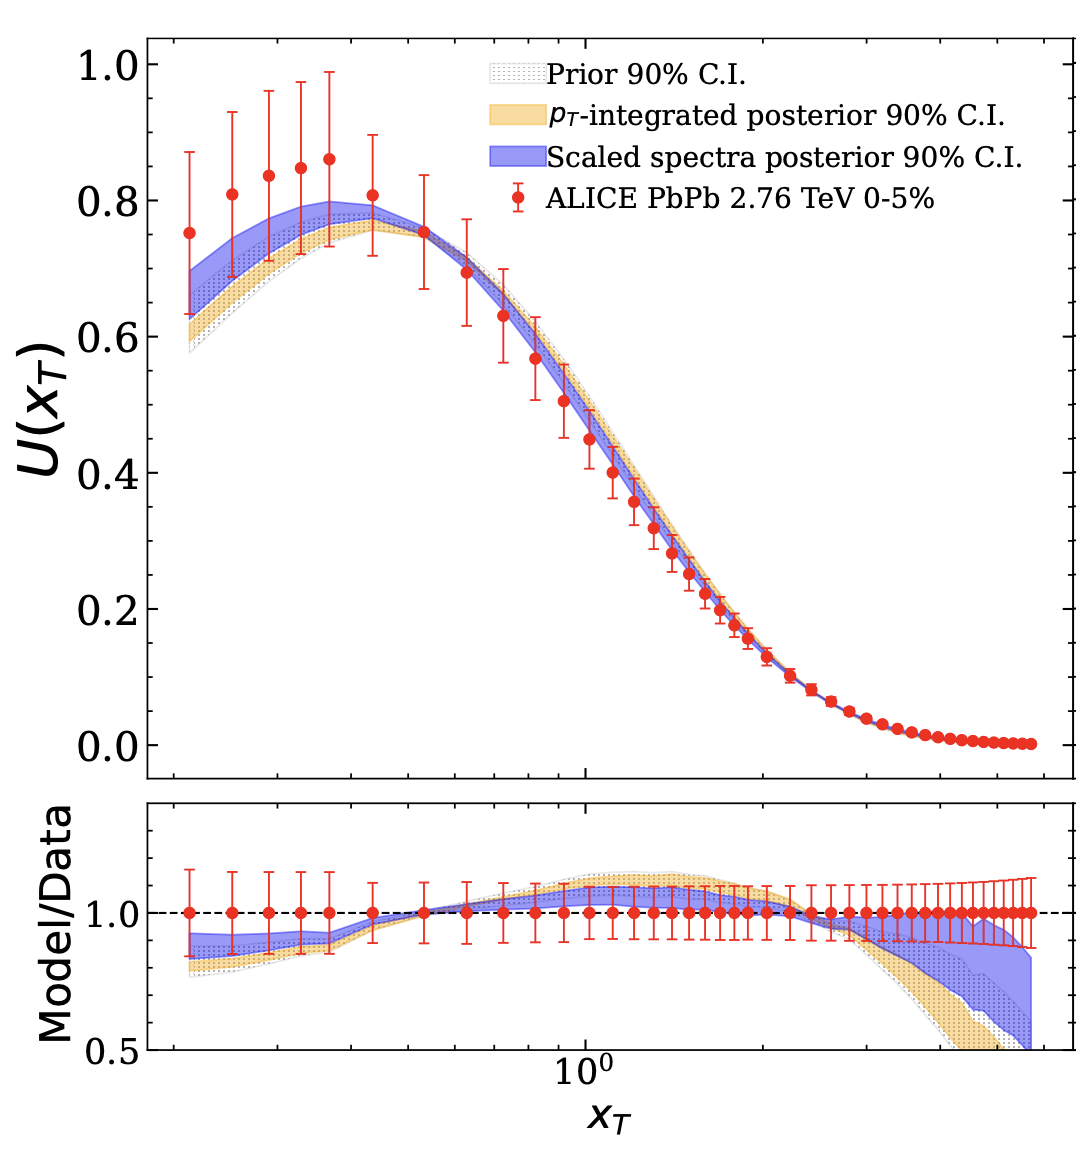
\includegraphics[width=\linewidth]{img/universal_scaled_spectra.png}

\vspace{0.1cm}

\tiny
Identified-particle spectra collapse onto a universal curve after rescaling.
{\tiny
Domingues \& Luzum, arXiv:2603.15891 (2026).
}
%====================================================
% RIGHT
%====================================================

\column{0.52\textwidth}

\small

\textbf{Motivation}

\begin{itemize}
    \item Remove trivial dependence on particle yield.
    \item Remove the characteristic momentum scale.
    \item Compare only the \textbf{shape} of the spectra.
\end{itemize}

\vspace{0.2cm}

The transverse momentum is rescaled as

\[
x_T=\frac{p_T}{\langle p_T\rangle},
\]

and the corresponding scaled spectrum is

\[
U(x_T)
=
\frac{\langle p_T\rangle}{N}
\frac{dN}{dp_T}
=
\frac{1}{N}
\frac{dN}{dx_T}.
\]
\end{columns}

\scriptsize
After this normalization, spectra from different collision centralities become nearly universal.



\end{frame}

%--------------------------------------------------------
